\subsection{Исходная функция}
Рассмотрим гармоническую функцию $f(t)$:
\begin{equation}
    f(t) = 3 \sin(2\pi x + \pi) + 2\sin(6 \pi x - 5)
\end{equation}
\def\num{1}
Ее график приведен на рисунке \ref{fig:source_func\num}.
\begin{figure}[ht!]
    \centering
    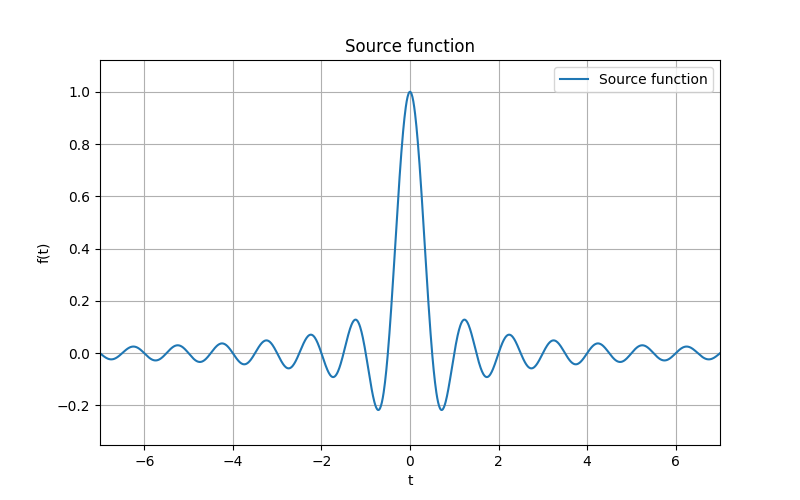
\includegraphics[width=\textwidth]{plots/interpolation_\num/source_func.png}
    \caption{Исходная функция}
    \label{fig:source_func\num}
\end{figure}

Рассмотрим ее \textit{сэмплированный} с периодом $\Delta t = 1/8$ секунды сигнал. График сигнала приведен на рисунке \ref{fig:sampled_func\num}.
\begin{figure}[ht!]
    \centering
    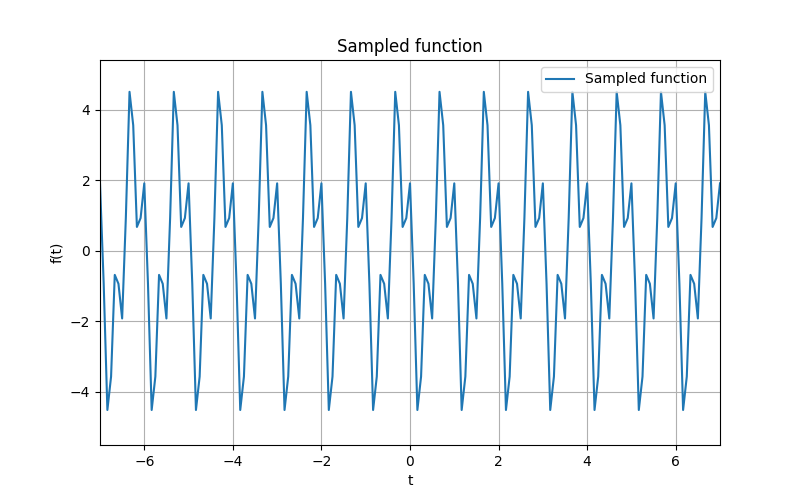
\includegraphics[width=\textwidth]{plots/interpolation_\num/sampled_func.png}
    \caption{Сэмплированный сигнал}
    \label{fig:sampled_func\num}
\end{figure}

И их сравнительный график приведен на рисунке \ref{fig:source_sampled_func\num}.
\begin{figure}[ht!]
    \centering
    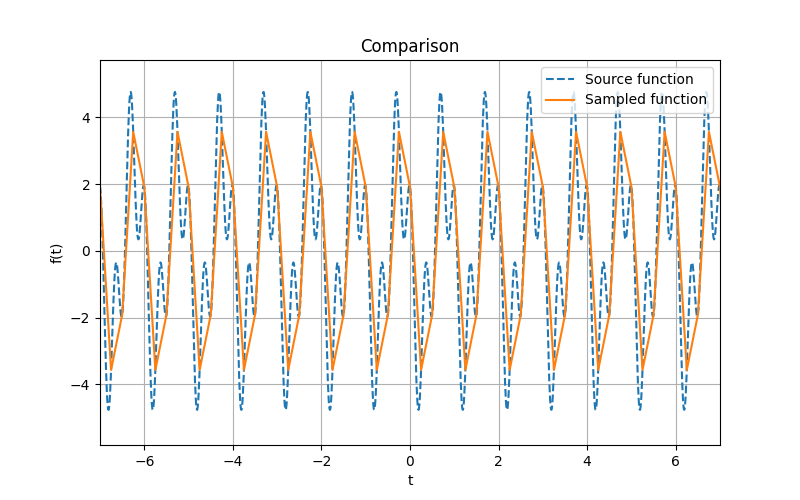
\includegraphics[width=\textwidth]{plots/interpolation_\num/cmp_func.png}
    \caption{Исходная и сэмплированная функции}
    \label{fig:source_sampled_func\num}
\end{figure}

\subsection{Восстановление}
Теперь попробуем восстановить начальную функцию, имея только сэмплированный сигнал. Для этого воспользуемся методом интерполяции: 
\begin{equation}
    f(t) = \sum_{-\infty}^{\infty} f(t_n) \cdot sinc\left(2B{t - t_n}\right)
\end{equation}

В результате ее применения получим график, приведенный на рисунке \ref{fig:interpolated_func\num}.
\begin{figure}[ht!]
    \centering
    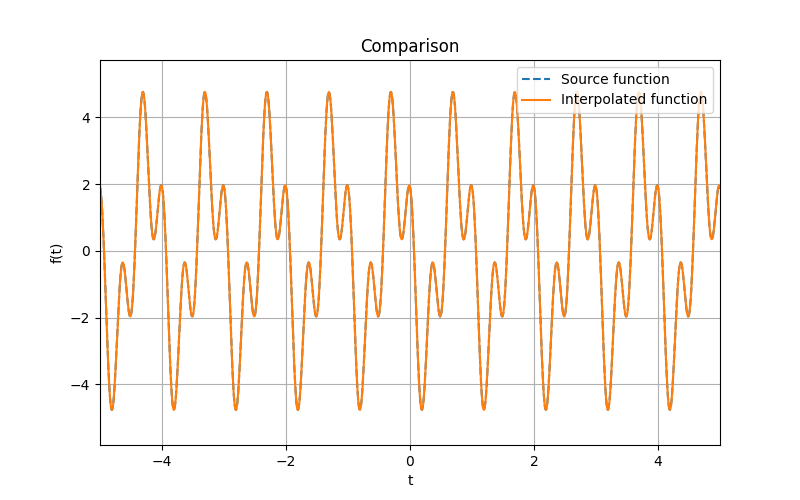
\includegraphics[width=\textwidth]{plots/interpolation_\num/cmp_func_interpolated.png}
    \caption{Восстановленная функция ($\Delta t = 1/8$)}
    \label{fig:interpolated_func\num}
\end{figure}

Видно, что функция восстановилась правильно даже при условии того, что в программной реализации нельзя 
брать бесконечную сумму. В своей программе я брал сумму от $-500$ до $500$.

\subsection{Вливание шага дискретизации}
\def\num{2}
Теперь попробуем влиять на шаг дискретизации. Пусть $\Delta t = 1/4$ секунды. График сэмплированной функции приведен на рисунке \ref{fig:source_sampled_func\num}.
\begin{figure}[ht!]
    \centering
    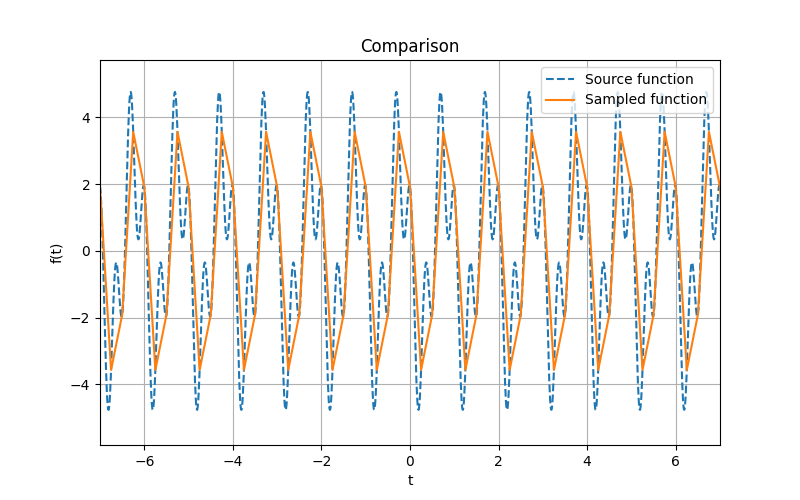
\includegraphics[width=\textwidth]{plots/interpolation_\num/cmp_func.png}
    \caption{Исходная и сэмплированная функции}
    \label{fig:source_sampled_func\num}
\end{figure}

График восстановленной функции приведен на рисунке \ref{fig:interpolated_func\num}.
\begin{figure}[ht!]
    \centering
    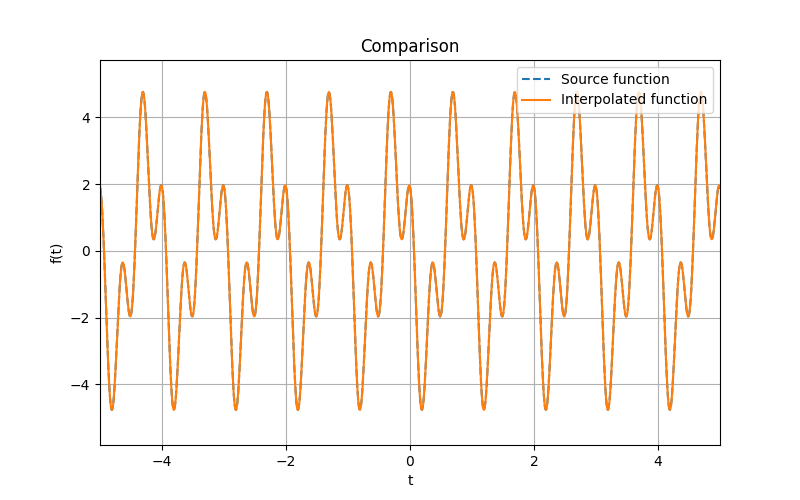
\includegraphics[width=\textwidth]{plots/interpolation_\num/cmp_func_interpolated.png}
    \caption{Восстановленная функция ($\Delta t = 1/4$)}
    \label{fig:interpolated_func\num}
\end{figure}

Тут уже видно, что функция восстановилась не так хорошо, как в предыдущем случае. Это связано с тем, 
что период дискретизации увеличился и стал больше, чем $1/2B$

\def\num{3}
Также возьмем шаг дискретизации $\Delta t = 1/10$ секунды. График сэмплированной функции приведен на рисунке \ref{fig:source_sampled_func\num}.
\begin{figure}[ht!]
    \centering
    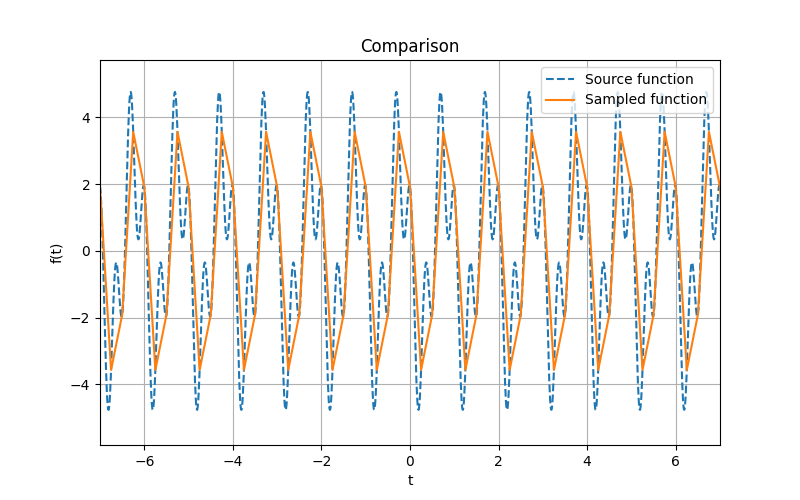
\includegraphics[width=\textwidth]{plots/interpolation_\num/cmp_func.png}
    \caption{Исходная и сэмплированная функции}
    \label{fig:source_sampled_func\num}
\end{figure}

График восстановленной функции приведен на рисунке \ref{fig:interpolated_func\num}.
\begin{figure}[ht!]
    \centering
    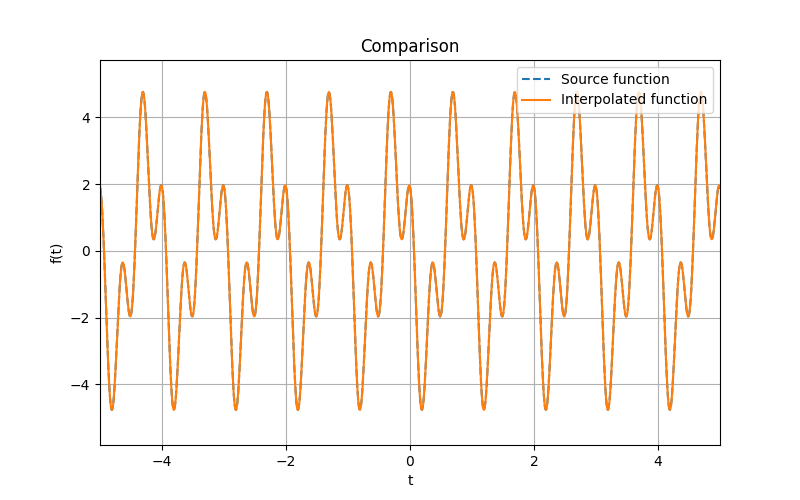
\includegraphics[width=\textwidth]{plots/interpolation_\num/cmp_func_interpolated.png}
    \caption{Восстановленная функция ($\Delta t = 1/4$)}
    \label{fig:interpolated_func\num}
\end{figure}

Видно, что при таком шаге дискретизации функция восстановилась правильно.

Таким образом, можно сделать вывод, что шаг дискретизации должен быть меньше $1/2B$ для корректного восстановления функции, что
соответствует теореме Найквиста-Шеннона-Котельникова.

\subsection{Сэмплирование sinc}
\def\num{4}
Теперь попробуем сэмплировать sinc-функцию. Пусть $f(t) = sinc(2\pi t)$. График этой функции приведен на рисунке \ref{fig:source_func\num}.
\begin{figure}[ht!]
    \centering
    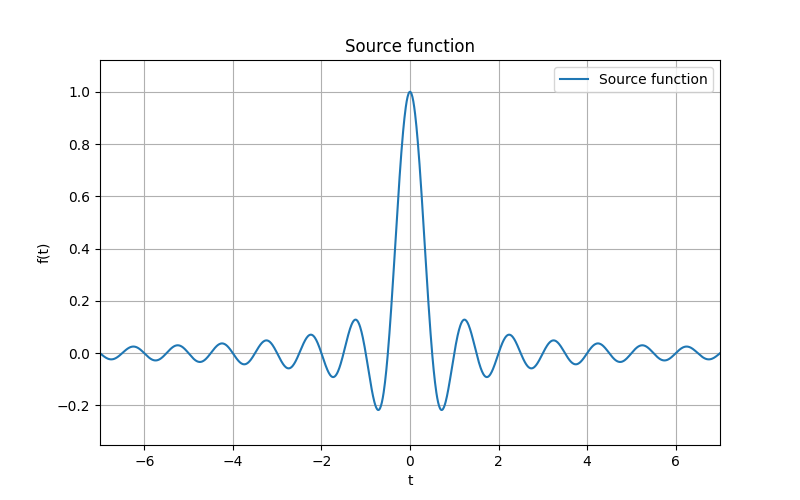
\includegraphics[width=\textwidth]{plots/interpolation_\num/source_func.png}
    \caption{Исходная функция}
    \label{fig:source_func\num}
\end{figure}

Сэмплированная в шагом $\Delta t = 1/4$ секунды функция приведена на рисунке \ref{fig:sampled_func\num}.
\begin{figure}[ht!]
    \centering
    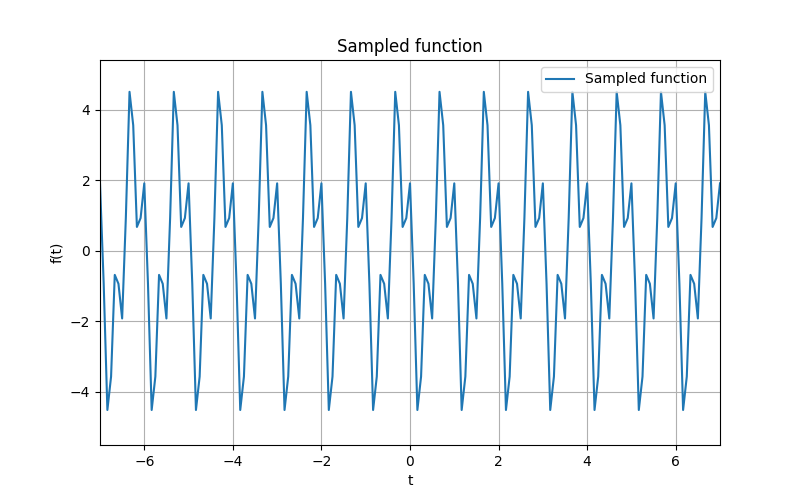
\includegraphics[width=\textwidth]{plots/interpolation_\num/sampled_func.png}
    \caption{Сэмплированный сигнал}
    \label{fig:sampled_func\num}
\end{figure}

Сравнительный график приведен на рисунке \ref{fig:source_sampled_func\num}.
Образ исходной функции приведен на рисунке \ref{fig:image\num}.
\begin{figure}[ht!]
    \centering
    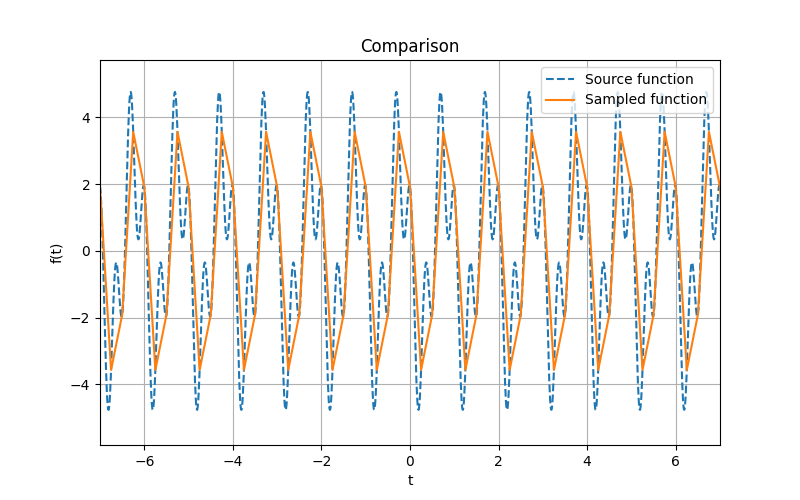
\includegraphics[width=\textwidth]{plots/interpolation_\num/cmp_func.png}
    \caption{Исходная и сэмплированная функции}
    \label{fig:source_sampled_func\num}
\end{figure}

\begin{figure}[ht!]
    \centering
    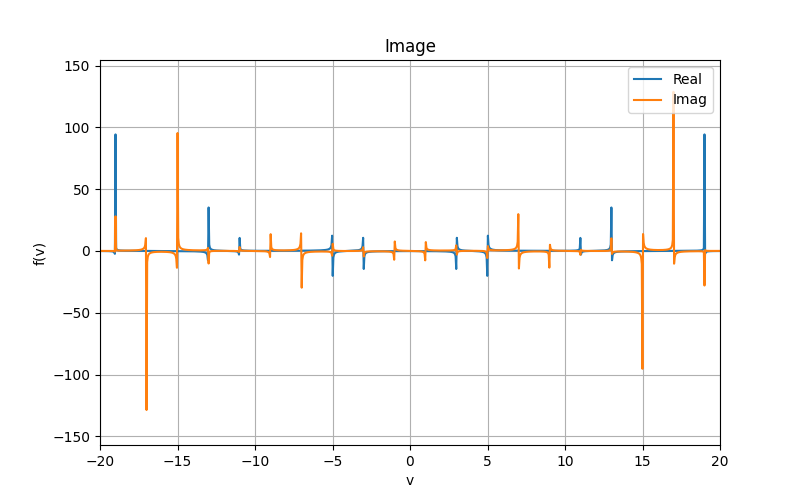
\includegraphics[width=\textwidth]{plots/interpolation_\num/image.png}
    \caption{Образ исходной функции}
    \label{fig:image\num}
\end{figure}

Как и ожидалось теоретически -- образ кардинального синуса -- это прямоугольная периодическая функция. 
Один период функции находится на отрезке $[-1, 1]$. Таким образом, восстановление функции без потерь возможно при значениях менее $\Delta t = 1/2$.
Восстановленная функция приведена на рисунке \ref{fig:interpolated_func\num}.
\begin{figure}[ht!]
    \centering
    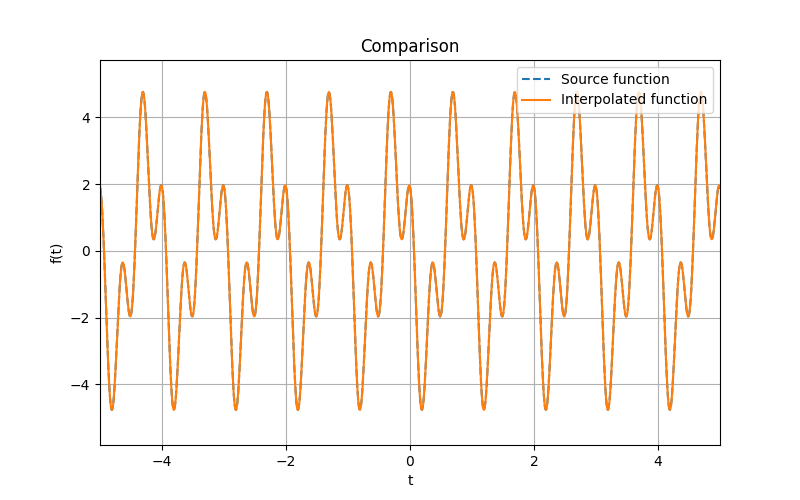
\includegraphics[width=\textwidth]{plots/interpolation_\num/cmp_func_interpolated.png}
    \caption{Восстановленная функция ($\Delta t = 1/4$)}
    \label{fig:interpolated_func\num}
\end{figure}

Образ восстановленной функции приведен на рисунке \ref{fig:restored_image\num}.
\begin{figure}[ht!]
    \centering
    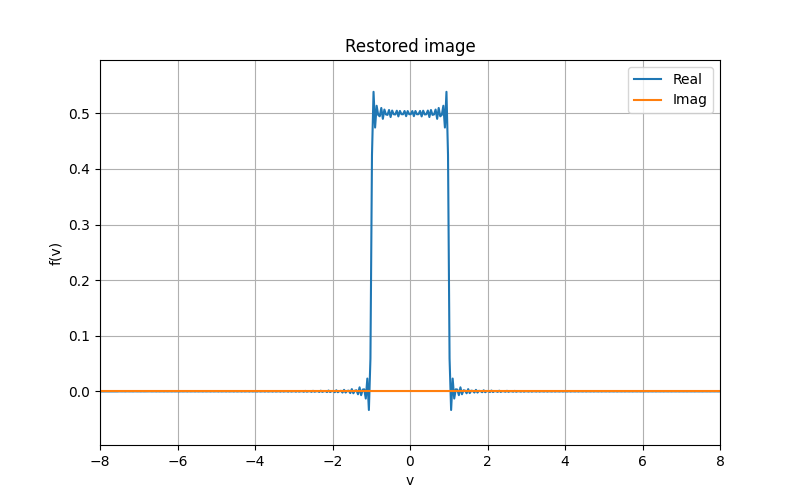
\includegraphics[width=\textwidth]{plots/interpolation_\num/restored_image.png}
    \caption{Образ восстановленной функции}
    \label{fig:restored_image\num}
\end{figure}

Образ восстановленной функции уже не является периодическим. Это связано с тем, что восстановленная 
функция уже не является дискретной, в отличие от сэмплированной. 

\def\num{5}
График функции, восстановленной из сэмплов с большим шагом, приведен на рисунке \ref{fig:interpolated_func\num}.
\begin{figure}[ht!]
    \centering
    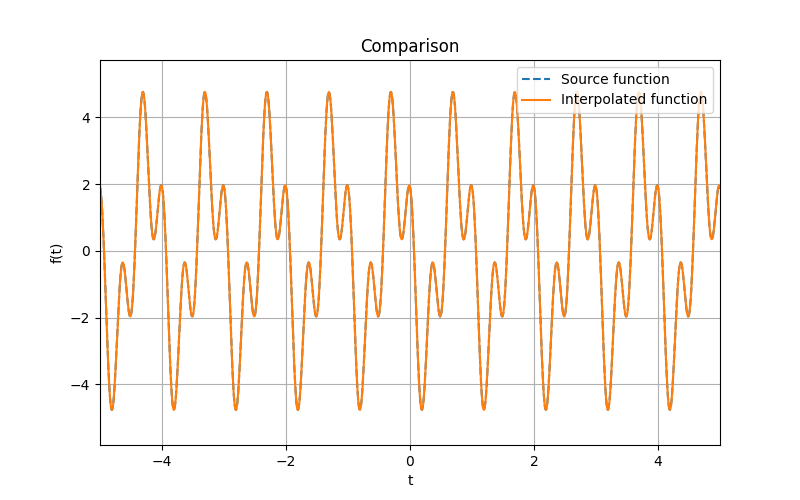
\includegraphics[width=\textwidth]{plots/interpolation_\num/cmp_func_interpolated.png}
    \caption{Восстановленная функция ($\Delta t = 1/2$)}
    \label{fig:interpolated_func\num}
\end{figure}

Как и ожидалось теоретически, функция восстановилась неправильно. Это связано с тем, что шаг дискретизации равен $1/2B$, а для корректного восстановления функции он должен быть меньше $1/2B$.